\documentclass[11pt]{article}
\usepackage[utf8]{inputenc}
\usepackage[french]{babel}
\usepackage{graphicx}
\usepackage[T1]{fontenc}
%\usepackage{amss}
\usepackage{amsmath}
\usepackage{amsfonts}
\usepackage{amssymb}

\newcommand\comment{}
\def\N{\mathbb N}
\def\R{\mathbb R}
\def\Q{\mathbb Q}
\def\Z{\mathbb Z}
\begin{document}
\title{PARTIEL I31, 2015\\Documents autorisés ???}
\date{}\maketitle



\section{Euclide et Bézout}

\smallskip

\begin{enumerate}
\item  En utilisant l'algorithme d'Euclide étendu, calculez le pgcd de 330 et 210 ainsi que les coefficients de Bezout:
$$u\in \Z, v\in \Z \ tels \ que \ 330u+210v=\mbox{PGCD}(330, 210)$$

Complétez le tableau ci-dessous.


\item Donnez une formule avec un paramètre permettant de générer toutes les paires d'entiers  $(u, v)$ telles
que $330u+210v=\mbox{PGCD}(330, 210)$.
\end{enumerate}

\medskip
\begin{tabular}{|p{2cm}|p{2cm}|p{2cm}|p{2cm}|p{2cm}|p{2cm}|p{2cm}|}
\hline a & b & r=b\%a & q=pgcd(a,b) & u & v\\ 
\hline 330 & 210  &   &   &   & \\
&    &   &   &   & \\
\hline   &    &   &   &   & \\
&    &   &   &   & \\
\hline   &    &   &   &   & \\
 &    &   &   &   & \\
\hline   &    &   &   &   & \\
&    &   &   &   & \\
\hline   &    &   &   &   & \\
 &    &   &   &   & \\
\hline
\end{tabular}




\section{Quizz}

\begin{enumerate}
\item Citez deux problèmes indécidables en informatique.

\item  Quand dit-on qu'un problème est difficile en informatique.

\item  Citez deux problèmes solubles en informatique, mais difficiles.

\item  Donnez deux algorithmes efficaces pour trier des nombres (\textbf{flottants ?}), en utilisant des comparaisons. Indiquez la complexité de ces deux algorithmes.

\item   Donnez le nom de trois algorithmes calculant les plus courts chemins dans un graphe.
\end{enumerate}

\section{Ordonnancement}

\begin{center}
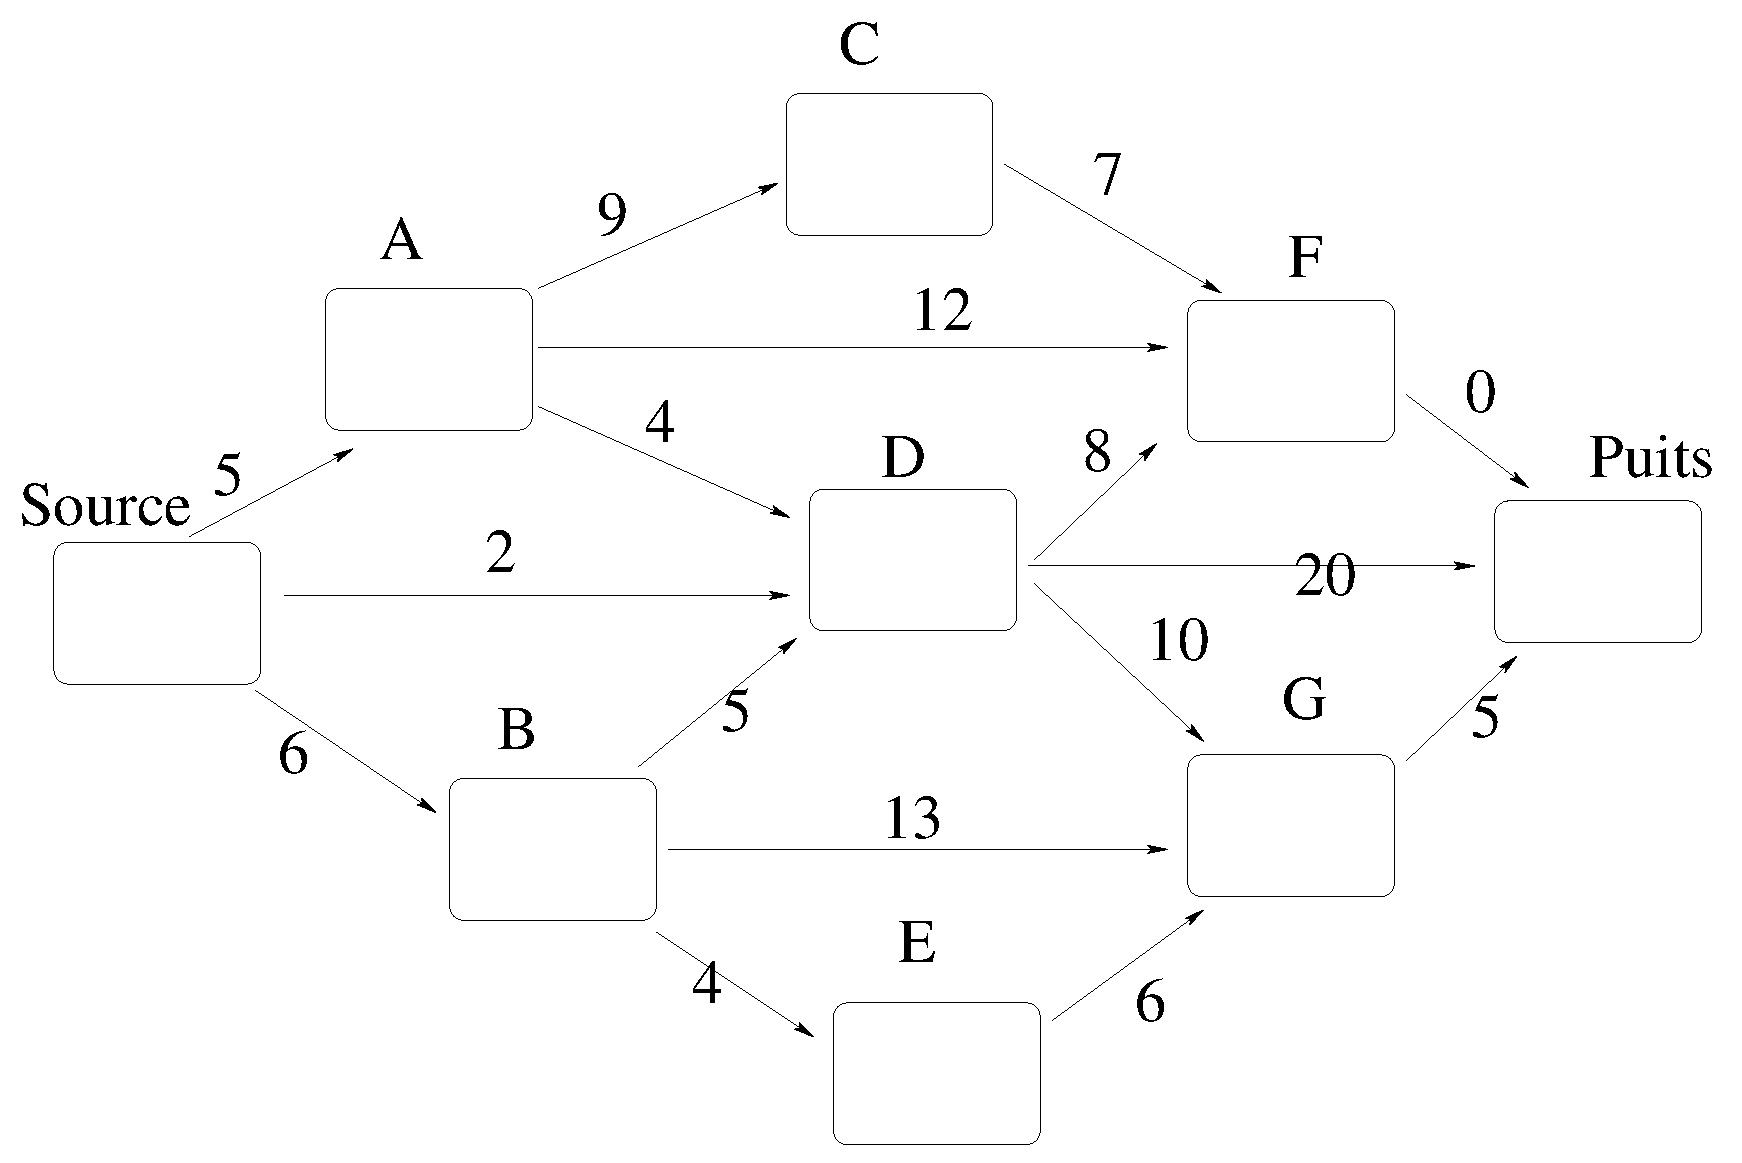
\includegraphics[width=0.7\linewidth]{critique.eps}
\end{center}

\textbf{ajouter 0-0 et 5-7 dans les deux tâches du début ?}

Etant donnée la description des tâches donnée ci-dessus: 

\begin{enumerate}

\item 
En calculant de SOURCE vers PUIT, complétez les dates au plus tôt (comme par exemple 0- et 5-).


Puis en calculant de  PUIT vers SOURCE, complétez les dates au plus tard (comme par exemple -0 et -7).

Soulignez le chemin critique.


\item Que faire si le graphe a plusieurs sommets sources (ou puits) ?

\item  Vous pouvez supposer que le graphe est acyclique, qu'il a un seul sommet source, un seul sommet puits, et que les durées sur les arcs sont non négatives.
Donnez la définition, en français, de la date au plus tôt. 
\textbf{Prévoyez bien tous les cas.?}

\item   Donnez la définition, en français, de la date au plus tard.

\item   Quand un sommet est-il critique~?

\end{enumerate}

\section{Dessinez le graphe d'un jeu de Nim}
Deux joueurs jouent à tour de rôle (Albert commence, Bertrand joue en second). Sur la table, il y a trois tas de pions~:
deux tas de 2 pions, et un tas de 1.

\smallskip
Chacun des joueurs choisit un tas (non vide) et  un seul,
et en retire un nombre entier  non nul  de pions~; il peut retirer  tous les pions du tas s'il le souhaite.

\smallskip
Le premier joueur qui ne peut plus retirer de pions
a perdu, ou, le premier joueur qui enlève tous les pions restant dans le dernier tas a gagné. 

\medskip
Vous utiliserez une représentation des états par niveaux: le niveau $n$ contient les états où la somme des nombres de pions vaut $n$ ($0 \le n \le 6 $). Un seul des états équivalents est représenté ($(2, 1, 1)=(1, 2, 1)=(1, 1, 2)$) et les $0$ inutiles sont éliminés.

Par exemple le niveau 2 contient
les états $(1, 1), (2)$. 

 \begin{enumerate}
\item  Sur le schéma des états par niveaux qui vous est fourni, indiquez  les sommets G pour gagnant, ou P pour perdant.

Un sommet est gagnant si le joueur qui y arrive peut toujours gagner, quels que soient les coups joués par l'adversaire.

Un sommet est perdant si ...

\item  Quel joueur, Albert ou Bertrand, est sûr de gagner, s'il joue intelligemment, bien sûr~?

\item Sur le schéma des états par niveaux qui vous est fourni, dessinez le graphe des coups possibles~; chaque état  est représenté par un sommet~; un arc va d'un sommet $s$ à un sommet $t$ quand il est possible de passer en un coup de $s$ à $t$. 


\item  \textbf{Décrivez l'algorithme que vous avez utilisé.?}


\item  Dans un graphe orienté acyclique (c'est le cas ici), un noyau $N$ est 
un sous-ensemble de sommets du graphe tel que~: si $s$ est dans $N$, tous ses voisins sont hors de $N$~; si $s$ est hors de $N$, il existe au moins un arc vers un sommet $t$ qui se trouve dans $N$. 

Quel est le lien avec le problème précédent~? 

\end{enumerate}


\end{document}
